%% Beginning of file 'sample7.tex'
%%
%% Version 7. Created January 2025.  
%%
%% AASTeX v7 calls the following external packages:
%% times, hyperref, ifthen, hyphens, longtable, xcolor, 
%% bookmarks, array, rotating, ulem, and lineno 
%%
%% RevTeX is no longer used in AASTeX v7.
%%
\documentclass[linenumbers,trackchanges]{aastex7}
%%
%% This initial command takes arguments that can be used to easily modify 
%% the output of the compiled manuscript. Any combination of arguments can be 
%% invoked like this:
%%
%% \documentclass[argument1,argument2,argument3,...]{aastex7}
%%
%% Six of the arguments are typestting options. They are:
%%
%%  twocolumn   : two text columns, 10 point font, single spaced article.
%%                This is the most compact and represent the final published
%%                derived PDF copy of the accepted manuscript from the publisher
%%  default     : one text column, 10 point font, single spaced (default).
%%  manuscript  : one text column, 12 point font, double spaced article.
%%  preprint    : one text column, 12 point font, single spaced article.  
%%  preprint2   : two text columns, 12 point font, single spaced article.
%%  modern      : a stylish, single text column, 12 point font, article with
%% 		  wider left and right margins. This uses the Daniel
%% 		  Foreman-Mackey and David Hogg design.
%%
%% Note that you can submit to the AAS Journals in any of these 6 styles.
%%
%% There are other optional arguments one can invoke to allow other stylistic
%% actions. The available options are:
%%
%%   astrosymb    : Loads Astrosymb font and define \astrocommands. 
%%   tighten      : Makes baselineskip slightly smaller, only works with 
%%                  the twocolumn substyle.
%%   times        : uses times font instead of the default.
%%   linenumbers  : turn on linenumbering. Note this is mandatory for AAS
%%                  Journal submissions and revisions.
%%   trackchanges : Shows added text in bold.
%%   longauthor   : Do not use the more compressed footnote style (default) for 
%%                  the author/collaboration/affiliations. Instead print all
%%                  affiliation information after each name. Creates a much 
%%                  longer author list but may be desirable for short 
%%                  author papers.
%% twocolappendix : make 2 column appendix.
%%   anonymous    : Do not show the authors, affiliations, acknowledgments,
%%                  and author contributions for dual anonymous review.
%%  resetfootnote : Reset footnotes to 1 in the body of the manuscript.
%%                  Useful when there are a lot of authors and affiliations
%%		    in the front matter.
%%   longbib      : Print article titles in the references. This option
%% 		    is mandatory for PSJ manuscripts.
%%
%% Since v6, AASTeX has included \hyperref support. While we have built in 
%% specific %% defaults into the classfile you can manually override them 
%% with the \hypersetup command. For example,
%%
%% \hypersetup{linkcolor=red,citecolor=green,filecolor=cyan,urlcolor=magenta}
%%
%% will change the color of the internal links to red, the links to the
%% bibliography to green, the file links to cyan, and the external links to
%% magenta. Additional information on \hyperref options can be found here:
%% https://www.tug.org/applications/hyperref/manual.html#x1-40003
%%
%% The "bookmarks" has been changed to "true" in hyperref
%% to improve the accessibility of the compiled pdf file.
%%
%% If you want to create your own macros, you can do so
%% using \newcommand. Your macros should appear before
%% the \begin{document} command.
%%
\newcommand{\vdag}{(v)^\dagger}
\newcommand\aastex{AAS\TeX}
\newcommand\latex{La\TeX}
%%%%%%%%%%%%%%%%%%%%%%%%%%%%%%%%%%%%%%%%%%%%%%%%%%%%%%%%%%%%%%%%%%%%%%%%%%%%%%%%
%%
%% The following section outlines numerous optional output that
%% can be displayed in the front matter or as running meta-data.
%%
%% Running header information. A short title on odd pages and 
%% short author list on even pages. Note that this
%% information may be modified in production.
%%\shorttitle{AASTeX v7 Sample article}
%%\shortauthors{The Terra Mater collaboration}
%%
%% Include dates for submitted, revised, and accepted.
%%\received{February 1, 2025}
%%\revised{March 1, 2025}
%%\accepted{\today}
%%
%% Indicate AAS Journal the manuscript was submitted to.
%%\submitjournal{PSJ}
%% Note that this command adds "Submitted to " the argument.
%%
%% You can add a light gray and diagonal water-mark to the first page 
%% with this command:
%% \watermark{text}
%% where "text", e.g. DRAFT, is the text to appear.  If the text is 
%% long you can control the water-mark size with:
%% \setwatermarkfontsize{dimension}
%% where dimension is any recognized LaTeX dimension, e.g. pt, in, etc.
%%%%%%%%%%%%%%%%%%%%%%%%%%%%%%%%%%%%%%%%%%%%%%%%%%%%%%%%%%%%%%%%%%%%%%%%%%%%%%%%
%%
%% Use this command to indicate a subdirectory where figures are located.
%%\graphicspath{{./}{figures/}}
%% This is the end of the preamble.  Indicate the beginning of the
%% manuscript itself with \begin{document}.

\begin{document}

\title{Galactic Mergers and Evolution: Stellar Density and Sersic Profile Development Due to Tidal Forces}

%% A significant change from AASTeX v6+ is in the author blocks. Now an email
%% address is required for each author. This means that each author requires
%% at least one of the following:
%%
%% \author
%% \affiliation
%% \email
%%
%% If these three commands are not available for each author, the latex
%% compiler will issue an error and if you force the latex compiler to continue,
%% it will generate an incomplete pdf.
%%
%% Multiple \affiliation commands are allowed and authors can also include
%% an optional \altaffiliation to indicate a status, i.e. Hubble Fellow. 
%% while affiliations are indexed as footnotes, altaffiliations are noted with
%% with a non-numeric footnote that is set away from the numeric \affiliation 
%% footnotes. NOTE that if an \altaffiliation command is used it must 
%% come BEFORE the \affiliation call, right after the \author command, in 
%% order to place the footnotes in the proper location. Because non-numeric
%% symbols are used, \altaffiliation should be used sparingly.
%%
%% In v7 the \author command takes an optional argument which provides 
%% additional metadata about the author. Authors can provide the 16 digit 
%% ORCID, the surname (family or last) name, the given (first or fore-) name, 
%% and a name suffix, e.g. "Jr.". The syntax is:
%%
%% \author[orcid=0000-0002-9072-1121,gname=Gregory,sname=Schwarz]{Greg Schwarz}
%%
%% This name metadata in not shown, it is only for parsing by the peer review
%% system so authors can be more easily identified. This name information will
%% also be sent to the publisher so they can include it in the CROSSREF 
%% metadata. Including an orcid will hyperlink the author name to the 
%% author's ORCID page. Note that  during compilation, LaTeX will do some 
%% limited checking of the format of the ID to make sure it is valid. If 
%% the "orcid-ID.png" image file is  present or in the LaTeX pathway, the 
%% ORCID icon will appear next to the authors name.
%%
%% Even though emails are now required for each author, the \email does not
%% produce output in the compiled manuscript unless the optional "show" command
%% is used. For example,
%%
%% \email[show]{greg.schwarz@aas.org}
%%
%% All "shown" emails are show in the bottom left of the first page. Due to
%% space constraints, only a few emails should be shown. 
%%
%% To identify a corresponding author, use the \correspondingauthor command.
%% The command appends "Corresponding Author: " to the argument it appears at
%% the bottom left of the first page like the output from \email. 

\author[gname='Matthew', sname='Gilles']{Matthew Gilles}
\affiliation{University of Arizona}
\email[show]{matthewgilles@arizona.edu}  

%% Use the \collaboration command to identify collaborations. This command
%% takes an optional argument that is either a number or the word "all"
%% which tells the compiler how many of the authors above the command to
%% show. For example "\collaboration[all]{(DELVE Collaboration)}" wil include
%% all the authors above this command.
%%
%% Mark off the abstract in the ``abstract'' environment. 

%% Keywords should appear after the \end{abstract} command. 
%% The AAS Journals now uses Unified Astronomy Thesaurus (UAT) concepts:
%% https://astrothesaurus.org
%% You will be asked to selected these concepts during the submission process
%% but this old "keyword" functionality is maintained in case authors want
%% to include these concepts in their preprints.
%%
%% You can use the \uat command to link your UAT concepts back its source.

%% From the front matter, we move on to the body of the paper.
%% Sections are demarcated by \section and \subsection, respectively.
%% Observe the use of the LaTeX \label
%% command after the \subsection to give a symbolic KEY to the
%% subsection for cross-referencing in a \ref command.
%% You can use LaTeX's \ref and \label commands to keep track of
%% cross-references to sections, equations, tables, and figures.
%% That way, if you change the order of any elements, LaTeX will
%% automatically renumber them.

\section{Introduction}

The topic proposed for my research assignment is to investigate how the
surface density profiles of MW and M31 evolve during their galactic merger.
Both galaxies have a disk and bulge region with its own surface density. When
MW and M31 merge within the next seven billion years, these two regions will
interact with each other and combine. The dynamical forces, namely the tidal
forces, will influence the result of this merger and the ongoing evolution
of the two galaxies.

Density is a property of a galaxy that influences many different phenomena
related to galactic evolution \citep{Torrey_Cox_Kewley_Hernquist_2012}. By
observing the surface density of the galaxies as they merge over time we can
learn about how galactic mergers influence evolution. With how old the
universe is, it is difficult to see the whole picture that is galactic
evolution. A galactic merger can hopefully allow us to see how a galaxy
evolves in a shorter amount of time. We can also learn what type of galaxy is
formed from the merger of MW and M31 by analyzing its surface density.

We know that after MW and M31 merge, the merger remnant will have a
significantly larger radius that the original galaxies
\citep{van_der_Marel_Besla_Cox_Sohn_Anderson_2012}. With this, the surface
density after the merger should follow a distribution similar to a de
Vaucouleurs profile \citep{Brooks_Christensen_2016}. This means that the new
elliptical merger remnant will have its density scale with the radius to the
power of a quarter (outside of 1 kpc from the centre). Figure 1 shows the
particles originating from MW and M31 respectively after the merger. It
can be seen that the shape of the merger remnant consisting of MW and M31
should be elliptical when viewed face on.

%% The "ht!" tells LaTeX to put the figure "here" first, at the "top" next
%% and to override the normal way of calculating a float position.
%% The asterisk after "figure" tells the compiler to span multiple columns
%% if a two column style is selected.
\begin{figure*}[h!]
\centering
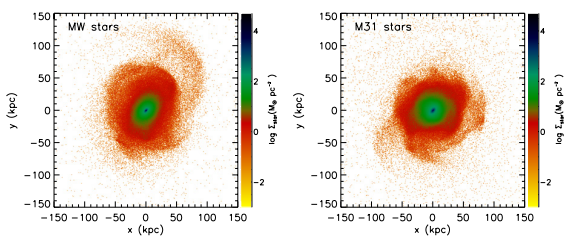
\includegraphics[scale=0.75]{van_der_Marel_et_al_Figure.png}
\caption{The distribution of particles at the end of the N-body simulation (t = 10 Gyr). Scale colour used to represent surface mass density. The centre of mass of each galaxy is at the highest-density position in its particle distribution \citep{van_der_Marel_Besla_Cox_Sohn_Anderson_2012}.
\label{fig:general}}
\end{figure*}

There are several questions relating to the evolution of the surface density
profiles during the galactic merger. A very good question is how will the
forces acting on the galaxies during the merger change their surface density
profiles. Hopefully, by analyzing the way the galaxy surface density changes
throughout this interaction and compare it to the initial densities and the
density of the merger remnant, we can learn more about how galactic mergers
and their density profiles impact galactic evolution. There is also the
question of how the merger will impact the form of the two galaxies. As
aforementioned, the merger remnant should be elliptical. The shape and density
of the merger remnant could help us learn how to more easily identify other
similar merger remnants. In the same vein, something must happen to the spiral
arms of MW and M31 as the galaxies go from a spiral classification to an
elliptical merger remnant. The tidal forces acting on the spiral arms cause
them to evolve in such a way that the arms lose their definition during the
merger.

\section{Proposal} \label{sec:style}

\subsection{This Proposal}

The question I will be answering is how the surface densities of the disks and bulges of MW and M31 evolve over the course of the galactic merger.

\subsection{Methods}

In order to answer this question, I will have to complete a number of steps
using the merger simulation. In general, I will look at surface density
profiles at various times for both MW and M31. As stated in the previous
subsection, I will look at both the evolution of the disk (i.e. particle type
2) and the bulge (i.e. particle type 3). I would like to analyze the two
galaxies at specific points in time. I will look at the initial conditions
(i.e. snapshot 000), the first close encounter at four gigayears (i.e.
snapshot 280), the time they separate after that encounter at five and a half
gigayears (i.e. snapshot 385), the time they merge at six and a half
gigayears (i.e. snapshot 455), and some time after the merger to see if there
are any changes (i.e. snapshot 700). These values were found using Figure 2
to look at the separation between MW and M31 during the galactic merger. At
these times, I will calculate the Sersic profile for each galaxy and find the
associated Sersic index that fits best. To do this, I will need to first
compute the centre of mass of each galaxy for the given snapshot. I will need
to do this for both particle types so that I can then find the surface density
for both the disk and the bulge. With the surface densities, I can then
calculate the Sersic profiles using the luminosity and effective surface
brightness. By over-plotting the surface density profile and sersic profile, I
can determine which Sersic index is most accurate.

\begin{figure*}[h!]
\centering
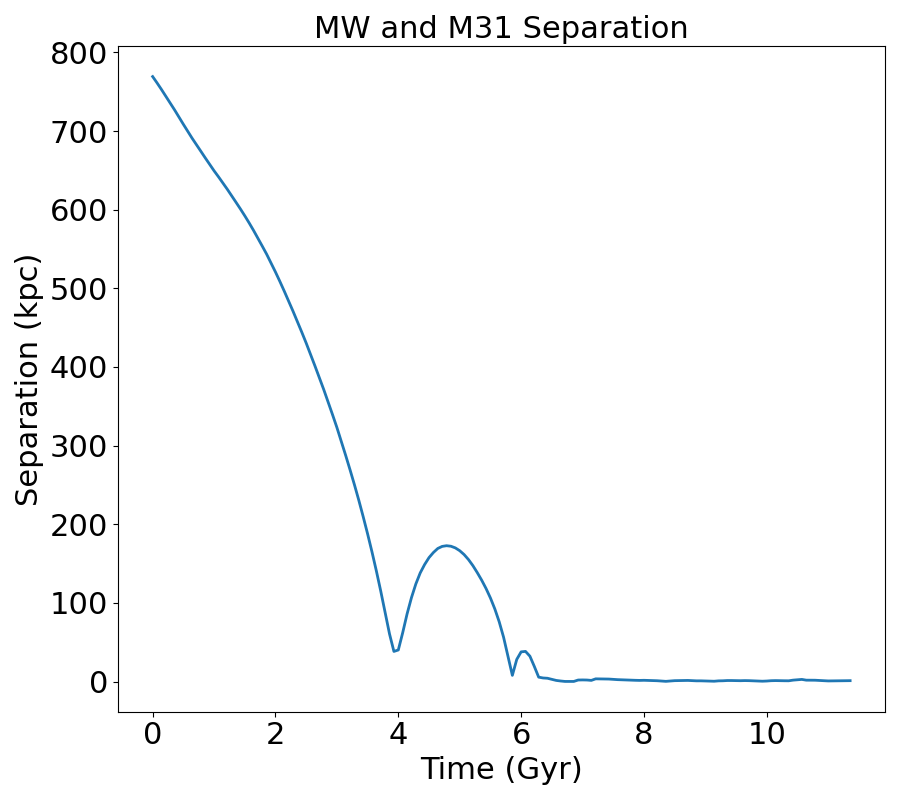
\includegraphics[scale=0.25]{MWM31RS.png}
\caption{Plot showing the radial separation between the centre of mass of MW and M31 in kpc at a given time in Gyr.
\label{fig:general}}
\end{figure*}

\subsection{Hypothesis}

I expect to find that the Sersic index at the end of the merger to be four.
This would fit with the merger remnant being elliptical in shape. It is also
likely that the Sersic indexes will vary between particle type as well as
snapshot number. This is due to the the bulge and disk having different
surface densities. 

%% For this sample we use BibTeX plus aasjournalv7.bst to generate the
%% the bibliography. The sample7.bib file was populated from ADS. To
%% get the citations to show in the compiled file do the following:
%%
%% pdflatex sample7.tex
%% bibtext sample7
%% pdflatex sample7.tex
%% pdflatex sample7.tex

\bibliography{ResearchAssignment2}{}
\bibliographystyle{aasjournalv7}

%% This command is needed to show the entire author+affiliation list when
%% the collaboration and author truncation commands are used.  It has to
%% go at the end of the manuscript.
%\allauthors

%% Include this line if you are using the \added, \replaced, \deleted
%% commands to see a summary list of all changes at the end of the article.
%\listofchanges

\end{document}

% End of file `ResearchAssignment2.tex'.
